\documentclass[11pt,a4paper]{article}
\usepackage[utf8]{inputenc}
\usepackage[italian]{babel}
\usepackage[margin=2cm]{geometry}
\usepackage{tabularx}
\usepackage{array}
\usepackage{graphicx}
\usepackage{xcolor}
\usepackage{booktabs}
\usepackage{graphicx}
\graphicspath{{images/}} 

\begin{document}
	
	\noindent
	\begin{minipage}{\textwidth}
		{\LARGE \textbf{Valutazione Euristica di Usabilità}} \\[0.5em]
		\textbf{Valutatore:} Nome Cognome \hfill \textbf{Data:} \today
	\end{minipage}
	\vspace{1.5em}
	\hrule
	\vspace{1.5em}
	
	\newcommand{\tabellaValutazioneEuristica}[6]{
		\noindent
		\begin{tabularx}{\textwidth}{|X|}
			\hline
			\begin{minipage}[t]{\linewidth}\raggedright
				\vspace{4pt}
				\textbf{Problema N\textsuperscript{o}:} #1 \hfill \textbf{Grado di Severità:} #5\\[4pt]
				\textbf{Posizione:} #2\\[6pt]
				\textbf{Descrizione:} \par
				#3\\[6pt]
				\textbf{Principi Violati:} \par
				#4
				\vspace{6pt}
			\end{minipage} \\ \hline

			\begin{minipage}[t]{\linewidth}\centering
				\vspace{4pt}
				\textbf{Screenshot:}
				\vspace{0.6em}
				
				#6
				\vspace{6pt}
			\end{minipage} \\ \hline
		\end{tabularx}
		\vspace{1em}
	}
	
	\tabellaValutazioneEuristica
	{-}
	{---}
	{---}
	{-}
	{\textbf{-}}
	{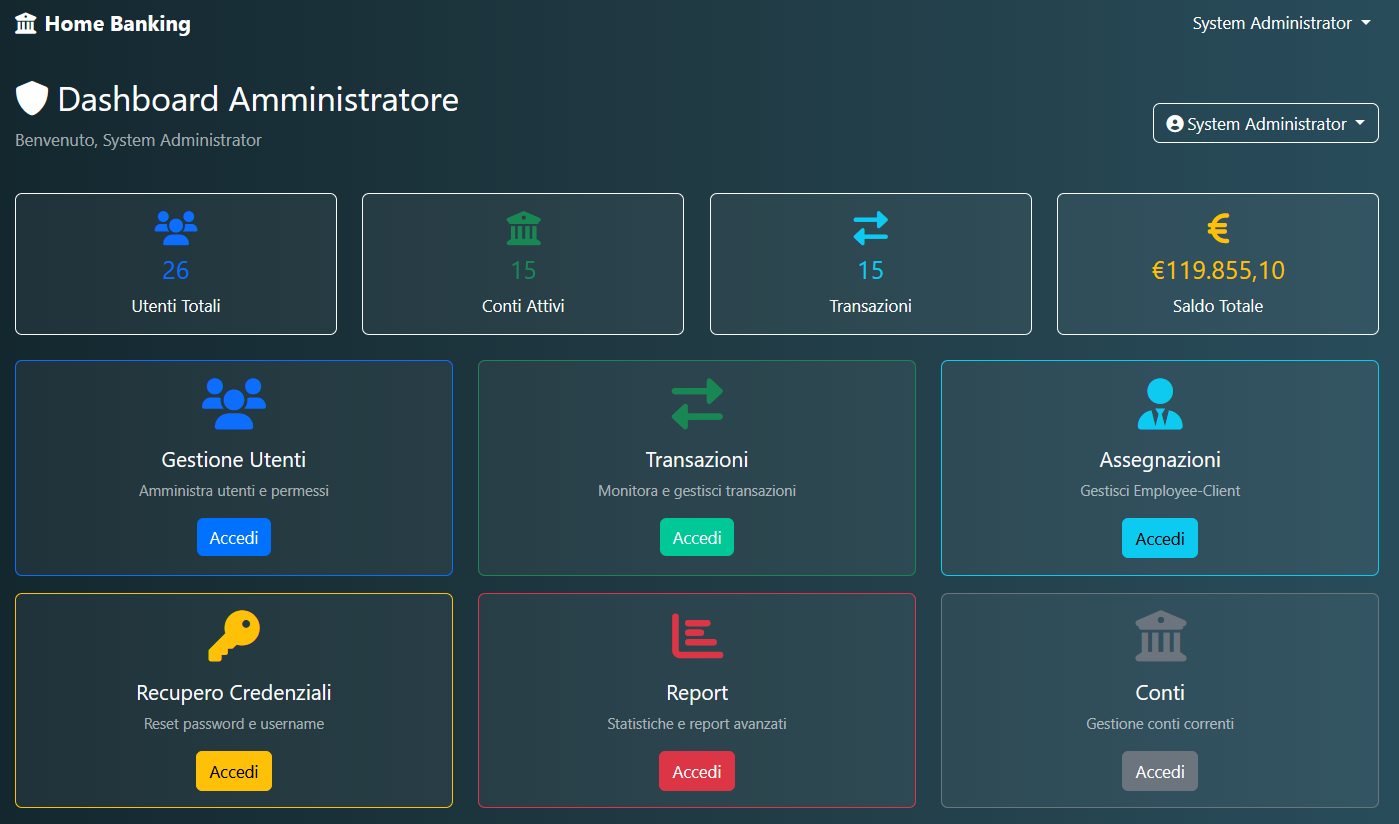
\includegraphics[width=0.75\linewidth]{example_screenshot.png}}
	
\end{document}